
% Theory part goes here %

% for numerated formulas
\newcommand{\formula}[3]
{
    \noindent#1\\[0.1cm]
    \begin{equation}\label{#2}
        #3
    \end{equation}
}

% for in-text math formulas
\newcommand{\mth}[1]
{
    \begin{math}
        #1
    \end{math}
}

% for rus letters in indexes
\newcommand{\ruB}[1]
{
    _{\text{#1}}
}

\section{Теория}

\subsection {Схема установки}

Схема установки представлена на рисунке 1.

\begin{center}

    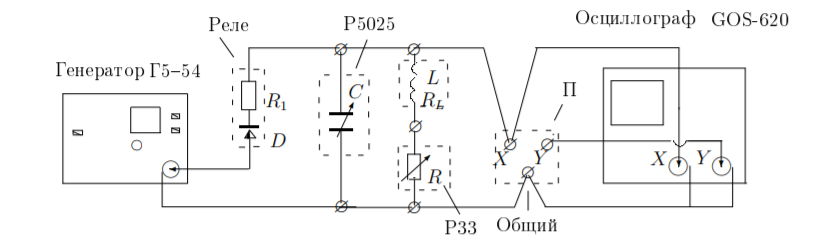
\includegraphics[scale=0.9]{324-scheme.png} \\
    \textit{Рис. 1. Схема установки}

\end{center}

\subsection {Исследуемые величины}

В работе планируется:

\begin{enumerate}
    \item Исследовать зависимость периода свободных колебаний контура от емкости. Согласно теории, зависимость должна иметь вид (Формула Томпсона):

    \formula
    {}
    {Tompson}
    {T = 2\pi \sqrt{LC}}

    \item Исследовать зависимость логарифмического декремента затухания от сопротивления. \\ Расчет логарифмического декремента затухания будет производиться по следующей формуле:

    \formula
    {}
    {Decrement}
    {\lambda = \ln\frac{W_k}{W_{k+n}}}

    \item Определить критическое сопротивление.

    \item Определить добротность контура.

\end{enumerate}